% !TEX root = main.tex
\chapter{Solid Phase Adsorption Toxin Tracking} \label{ch:spattss}

\section{Introduction}
Monitoring waterbodies for \gls{hab} require frequent visits to water sampling at a point in time can miss \gls{hab} events. Concentrations may fluctuate through time and sampling at a large interval may not capture the reality of the lake's condition. Solid Phase Adsorption Toxin Tracking (SPATT) is new unique method of monitoring waterbodies in a more time-integrative approach. SPATT is used as a bag or a sachet is filled with a porous resin inside a permeable bag.
SPATT is used in for monitoring other analyte of interest such as diarrhetic shellfish poisoning \cite{mackenzie_solid_2004}. %%%%%%%%%%%%NEED MORE CITATION$$$$$$$$
The SPATT bag  is submerged in a waterbody of interest for a period of time. During this period, free-floating compounds will adsorb onto the polymer beads.  SPATT can are then retrieved and analyzed for chemical analytes of interest. This technique can be useful if sampling frequency is financially limited.

\section{Methods}

The SPATT bag will be make with Nitex\footnote{Purchased from Dynamic Aqua-Supply Ltd.  \url{http://www.dynamicaqua.com/nitex.html}} and filled with HP-20\footnote{Purchased from Sigma Aldrich: CAS Number 9052-95-3}, a non-polar resin (styrene-divinylbenzene copolymer),
To construct the SPATT bags, a 1 meter x 5 centimeter strip of Nitex mesh were cut with sharp blade. The Nitex strip was sewn by folding half length-wise (or \emph{hot dog} style). With tape holding the fold, the end of the strip was sewn 0.5cm from the edge. Stitching design was tight to ensure no leakage of polymer beads.

9-10cm of sewn Nitex strips were cut and zip-tied about 0.5cm at one end. 3.00-3.01 grams of HP-20 resin was filled using a funnel. The other end is zip-tied once the Nitex bag is full. SPATT bags are activated by soaking in 100\% methanol for 24 hours under $4^\circ$C. Next the SPATTs were rinsed with Milli-Q water and then soaked for 24 hours in Milli-Q water under $4^\circ$C before deploying the SPATT bag in our target sample lakes.

At each lake site, two SPATT bags were loaded into a slotted PVC pipe. At each lake, a float was installed as described in section \ref{sampling}. SPATT are left for about a month at each lake. When SPATT are retrieved, they are carefully removed and rinsed with Milli-Q water and stored in a 15mL centrifuge vial with a plastic spacer on the bottom. SPATT are stored at $4^\circ$C during transport back to the lab. The SPATT are centrifuged at 8000rpm. The spacer allows liquid to pool on the bottom when centrifuged. When centrifuged, the SPATT bags are cut open and the resin is poured into a 50mL centrifuge tube. Milli-Q water is used to rinse the SPATT bags to effectively transfer all the resin. About 30mL of Milli-Q water is used. The solution is allowed to rest so the resin settles to the bottom. Using a pipet, the water is carefully decanted until the total volume is 5mL.  A solution of 80\% methanol with 10$\mu$M ammonium formate is added to the tube until the total volume is 45mL. The solution is gently mixed and then allowed to settle for 30 minutes. 3.5mL of the supernatant is transferred to glass vials and analyzed by the Westerick group. See section \ref{sc:lcms}

\section{Results}

Out of all 12 congeners, MC-LA, MC-LR, and MC-RR were the most frequently detected congener (see \ref{tab:spattcongener}). Microcystin concentrations from SPATT was mostly detected in lake Paradise, Intermediate Lake, Lake Cadillac and Wixom Lake. Comparing the average results from SPATT to the grab sample, we identified a major difference (see \ref{fig:spattbox}). When average concentration of MC from SPATT and grab sample is ordered by latitude, we found the relative mangitude of microcystin is higher found in the upper latitude of Michigan compared to regular grab sample. In our grab sample, Brighton, Pontiac, Wixom Lake and Lake Cadillac had high average MC with notable \gls{hab}.

\begin{figure}[!hp]
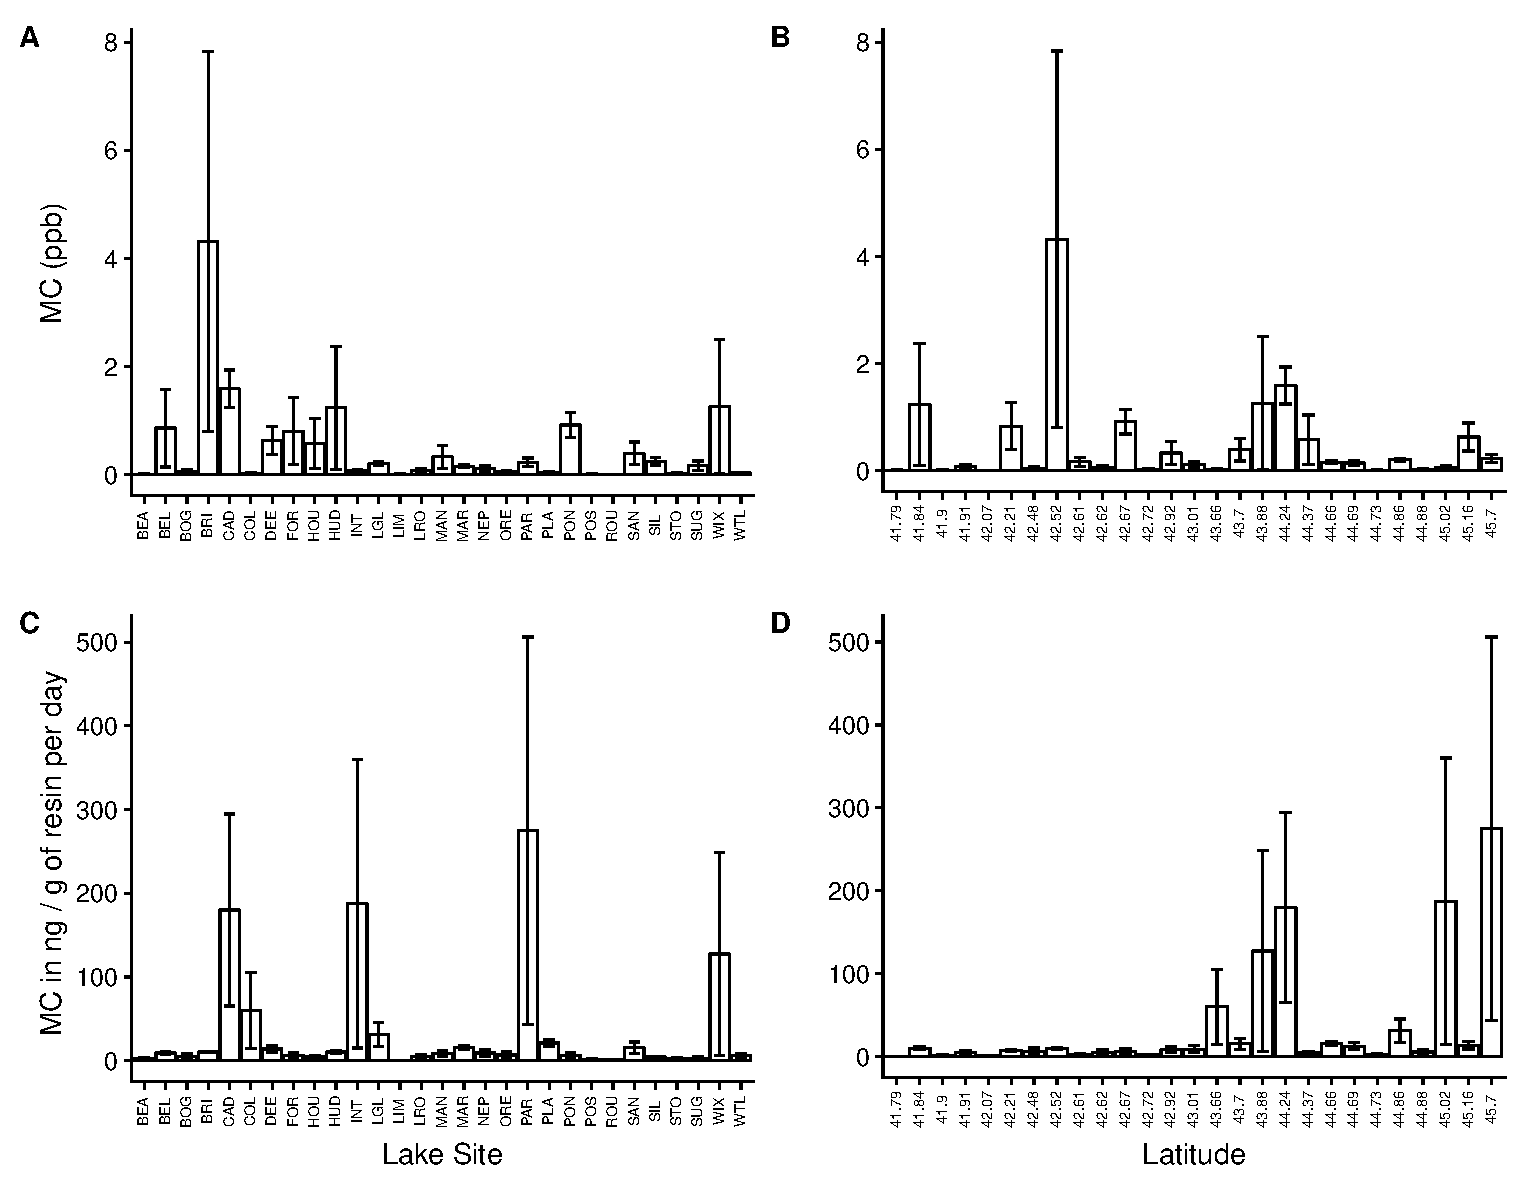
\includegraphics[width=\textwidth]{figures/spatttboxplotlake}
\caption{
Microcystin measured from SPATTS compared to grab sample: and Grab Samples. Average concentration of MC are plotted as bar graphs. Microcystin concentrations analyzed from grab sample are shown in figure (A) arranged by each lake and (B) arranged by latitude. Microcystin concentrations analyzed from SPATT samples are shown in figure (C) arranged by each lake and figure (D) arranged by latitude
}
\label{fig:spattbox}
\end{figure}

\begin{figure}[!ht]
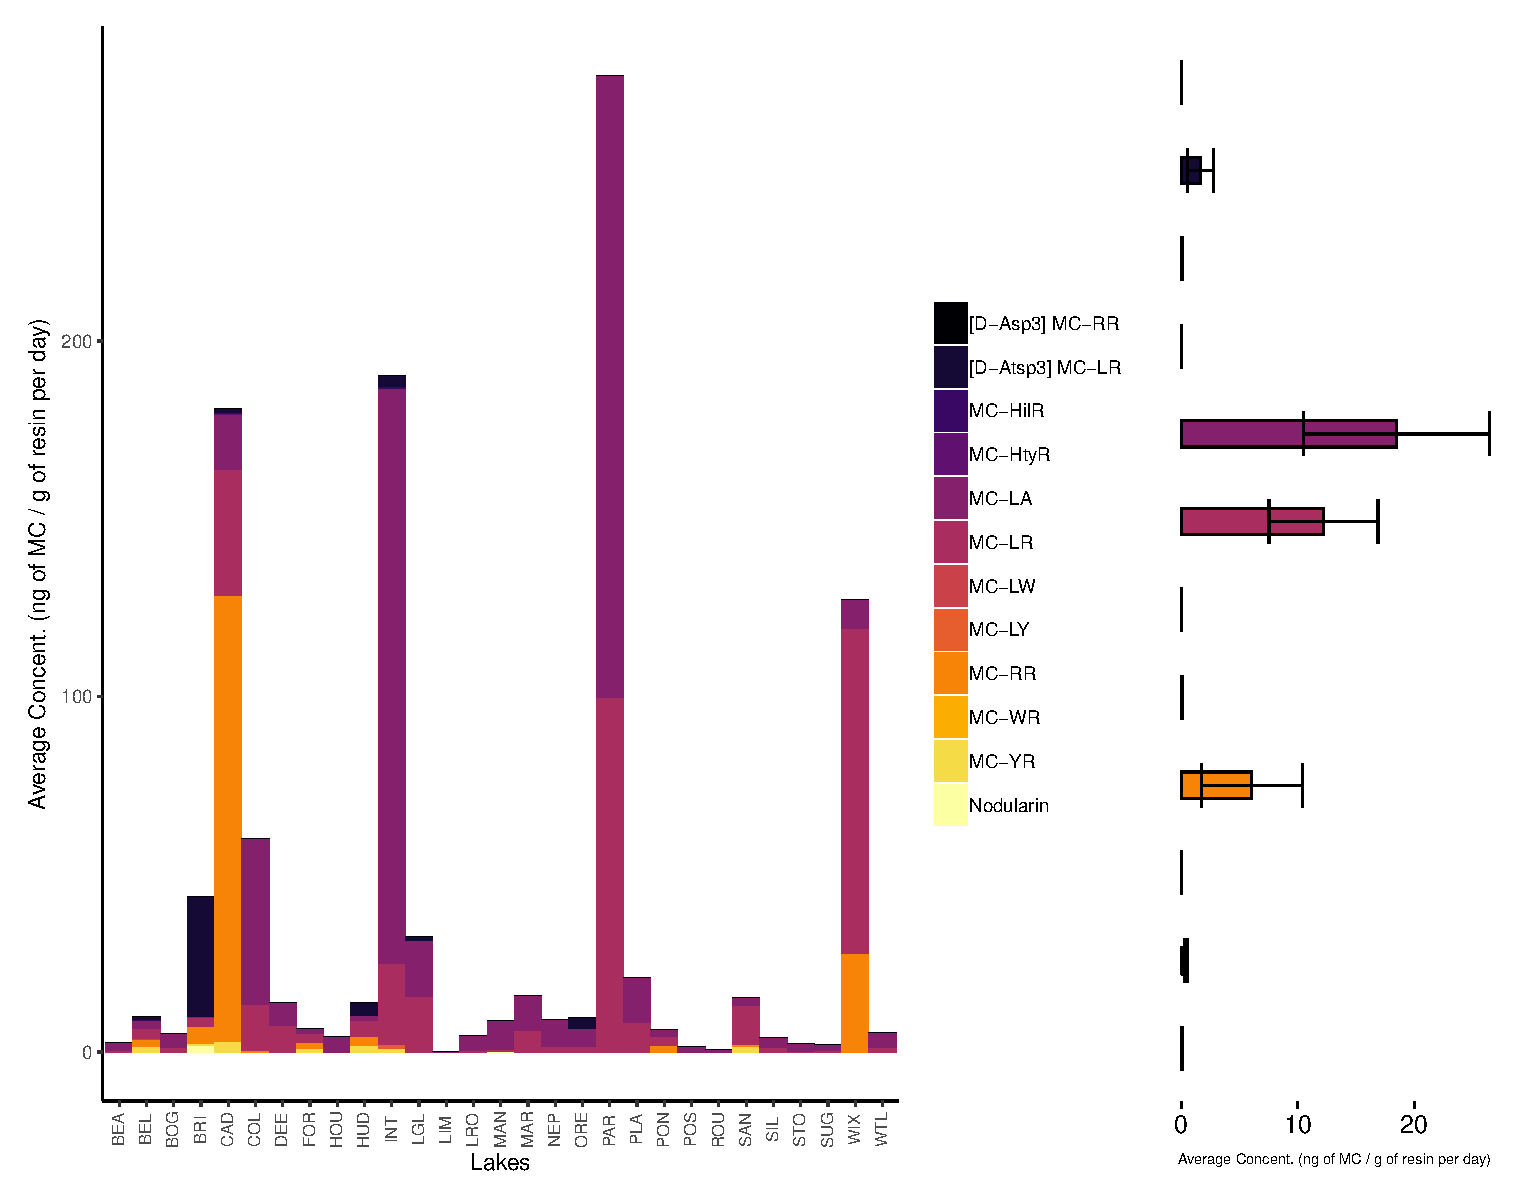
\includegraphics[width=\textwidth]{figures/barspatts}
\caption{Average MC congeners at each lake. Error bars represent one standard deviation of the mean}
\label{fig:barspatts}
\end{figure}

\begin{table}[!ht]
\centering
  \caption{Microcystin Congener from SPATT}
  \label{tab:spattcongener}
\begin{tabular}{@{\extracolsep{5pt}}lccccc}
\\[-1.8ex]\hline
\hline \\[-1.8ex]
Statistic & \multicolumn{1}{c}{N} & \multicolumn{1}{c}{Mean} & \multicolumn{1}{c}{St. Dev.} & \multicolumn{1}{c}{Min} & \multicolumn{1}{c}{Max} \\
\hline \\[-1.8ex]
{[D-Asp3]}MC-RR & 91 & ND & ND & ND & ND \\
MC-RR & 91 & 164 & 1,116 & ND & 10,380 \\
Nodularin & 91 & 2 & 17 & ND & 160 \\
MC-YR & 91 & 10 & 30 & ND & 145 \\
MC-HtyR & 91 & 0 & 2 & ND & 18 \\
MC-LR & 91 & 353 & 1,211 & ND & 8,146 \\
{[D-Asp3]}MC-LR & 91 & 2 & 10 & ND & 92 \\
MC-HilR & 91 & 1 & 6 & ND & 53 \\
MC-WR & 91 & 0 & 1 & ND & 7 \\
MC-LA & 91 & 534 & 2,063 & ND & 13,977 \\
MC-LY & 91 & 1 & 11 & ND & 101 \\
MC-LW & 91 & 0 & 0 & ND & 0 \\
MC-LF & 91 & 0 & 2 & ND & 18 \\
Total MC & 91 & 1,066 & 3,273 & ND & 22,124 \\
\hline \\[-1.8ex]
\multicolumn{6}{r}{Values are expressed as (ng of MC / gram of resin)} \\
\multicolumn{6}{r}{ND=No Detects} \\
\end{tabular}
\end{table}


\clearpage
\newpage

\section{Discussion}

The results from SPATT seemed to suggest the lakes we found to have low microcystin from our grab sample missed other \gls{hab}. When lakes were ordered by latitude, it also suggest lakes found in the upper latitude of Michigan may had higher frequency of \gls{hab}.

We suggest there is another factor that explains the higher magnitude of microcystin. We started to observe biofilm to accumulate on the SPATT bags. The biofilm was more notable in lakes that had significant blooms such as Brighton, Pontiac, and Wixom Lake. Initially we did not expect this would effect the capacity of the SPATT, but this data may suggest this. In our next year of survey we will test the hypothesis if the biofilm has a negative effect of microcystin adsorption. We may need to dispatch the SPATT bags more often to prevent biofilm to encase and clog the Nitex mesh bag.



